\documentclass[10pt,openany,a4paper]{article}
\usepackage{amsmath, amsfonts, amssymb, amsthm}
\usepackage{tikz, pgfplots, tkz-euclide,calc}
    \usetikzlibrary{patterns,snakes,shapes.arrows,arrows.meta}
\usepackage{fancyhdr}
\usepackage{enumerate,enumitem}
\usepackage{cancel}
\usepackage{varwidth}
\usepackage{array}
\usepackage{animate}
\usepackage{multirow,multicol}
\usepackage{hyperref}
\hypersetup{
    colorlinks=true,
    linkcolor=blue,
    filecolor=magenta,      
    urlcolor=cyan,
    pdftitle={Overleaf Example},
    pdfpagemode=FullScreen,
    }
\usepackage{graphicx}
\graphicspath{{C:/Users/teoso/OneDrive/Documents/Asisten Dosen & Lab/Asisten Laboratorium/Alpro 1/PPT/Graphicx/}{C:/Users/teoso/OneDrive/Documents/Tugas Kuliah/Template Math Depart/}}

% TAMBAHKAN PACKAGE SENDIRI KALAU KURANG

\usepackage{geometry}
\geometry{
	left = 20mm,
	right = 20mm,
	top = 30mm,
	bottom = 30mm,
}


\pagestyle{fancy}
\fancyhead{}
\fancyfoot{}
\fancyhead[r]{}
\fancyhead[l]{\fbox{\large{\textbf{SKPB - ITS}}}}
\renewcommand{\headrulewidth}{0pt}
\renewcommand{\footrulewidth}{0pt}

\newcommand{\R}{\mathbb{R}}
\newcommand{\N}{\mathbb{N}}
\newcommand{\C}{\mathbb{C}}
\newcommand{\Z}{\mathbb{Z}}
\newcommand{\Q}{\mathbb{Q}}
\newcommand{\cis}{\text{cis}}

\begin{document}

    \begin{center}
	{\underline{\textbf{\MakeUppercase{Evaluasi Tengah Semester Bersama Genap 2024/2025}}}}
    \end{center}

    \begin{center}
	\begin{tabular}{lcl}
		Mata kuliah/SKS & : & Kalkulus 1 ( SM234101 ) / 3 SKS\\
		Hari, Tanggal & : & Kamis, 12 Desember 2024\\
		Waktu & : & 13.30-15.10 WIB (100 menit)\\
		Sifat & : & Tertutup\\
		Kelas & : & 34-46, 107, 108
	\end{tabular}
    \end{center}
	
    \noindent\rule{\textwidth}{2.pt}
	
    \setlength{\parindent}{5pt}
    \setlength{\parindent}{5pt}
    \centering{Tuliskan: Nama, NRP, dan Nomor Kelas pada lembar jawaban Anda.}
    \setlength{\parindent}{5pt}
    \par \textbf{\MakeUppercase{dilarang membawa/menggunakan kalkulator dan alat komunikasi}}
    \centering{\textbf{\MakeUppercase{dilarang memberikan/menerima jawaban selama ujian}}}
    \par \centering{\textbf{"Setiap tindak kecurangan akan mendapat sanksi akademik."}}
    \noindent\rule{\textwidth}{2.pt}
    
	\begin{table}[h]
        \centering
        EAS Mengukur Kemampuan
        \begin{tabular}{|c|m{10.5cm}|c|c|}
            \hline
            CPL & CPMK & SOAL & BOBOT (\%) \\ \hline
            \multirow{5}{*}{2} 
            & CPMK-2 Mampu menentukan kekontinuan fungsi dan & 1 & 20 \\ \cline{3-4}
            & turunannya & 2 & 20 \\\cline{2-4}
            & CPMK-3 Mampu menghitung integral melalui teorema fundamental kalkulus & 3 & 20 \\ \cline{2-4}
            & CPMK-4 Mampu mengaplikasikan bentuk peubah kompleks dalam bentuk polar serta mencari akar-akar persamaannya & 4 & 20 \\ \cline{2-4}
            & CPMK-5 Mampu menerapkan konsep matriks untuk menyelesaikan sistem persamaan linier dan menentukan nilai eigen & 5 & 20 \\ \hline
        \end{tabular}
    \end{table}
    {\centering\textbf{SOAL}}
% SOAL DI SINI YAA
    \begin{enumerate}
        \item Diberikan kurva $y = \sqrt{x}$ untuk $0 \leq x \leq 3$. Dapatkan titik pada kurva yang memiliki jarak terdekat dengan titik $(2, 0)$.
    
    \item Diberikan fungsi $f(x) = \displaystyle\frac{x}{x - 2024}$.
    \begin{enumerate}
        \item Tentukan asimtot datar dan tegaknya (jika ada).
        \item Tentukan selang dimana fungsi $f(x)$ naik atau turun.
        \item Tentukan titik ekstrim relatif fungsi tersebut.
        \item Tentukan selang kecekungan fungsi $f(x)$ dan titik belok (jika ada).
        \item Sketsa grafiknya.
    \end{enumerate}

    \item Misalkan $F(x) = \displaystyle\int_{-1}^x \frac{1 + t^3}{1 + t^2} \, dt$. Dapatkan $F(-1)$, $F'(-1)$, dan $F''(-1)$.

    \item Nyatakan bilangan kompleks $\displaystyle z = \left(\frac{\left(1 + i\right)^{12}\left(1 + i\sqrt{3}\right)^{16}}{(-1 + i)^{32}}\right)$ dalam bentuk $z = a + bi$.

    \item Carilah nilai $x_3$ dari sistem persamaan linear berikut:
    \begin{align*}
        x_1 + 4x_3 + x_4 &= 11, \\
        2x_1 + 3x_3 + 2x_4 &= 12, \\
        5x_1 + x_2 + 2x_3 + x_4 &= 20, \\
        4x_1 + 6x_3 + x_4 &= 24,
    \end{align*}
    dengan menggunakan metode Cramer.
    \end{enumerate}
    \begin{center}
        \rule{0.28\textwidth}{2.pt}$\quad$\textbf{Selamat Mengerjakan}$\quad$\rule{0.28\textwidth}{2.pt}
    \end{center}

    \newpage
    \fancyhead[L]{\textit{Solution By: \hyperlink{https://github.com/TetewHeroez}{Tetew}}}
    \fancyfoot[R]{\animategraphics[autoplay,loop,width=0.1\textwidth]{15}{Kuru Kuru Herta/kuru kuru-}{0}{5}}
    {\centering\textbf{SOLUSI}}
    \renewcommand{\arraystretch}{1.5}
    \renewcommand{\headrulewidth}{1pt}
    \begin{enumerate}
        \item Pertama-tama dari soal kita tahu bahwa titik yang berada pada kurva memiliki koordinat $(x, \sqrt{x})$. Kemudian jarak antara titik $(x, \sqrt{x})$ dengan titik $(2, 0)$ dapat didefinsikan dengan
        \[D(x)= \sqrt{(x-2)^2 + (\sqrt{x} - 0)^2} = \sqrt{x^2 - 4x + 4 + x} = \sqrt{x^2 - 3x + 4}.\]
        Dapat dilihat bahwa $D(x)$ merupakan fungsi yang bergantung pada $x$ dengan interval $0 \leq x \leq 3$. Untuk mencari nilai minimum dari $D(x)$, kita cari titik stasioner dari $D(x)$ dengan mencari turunan pertama dari $D(x)$, yaitu
        \[D'(x) = \frac{2x - 3}{2\sqrt{x^2 - 3x + 4}} = 0 \implies x = \frac{3}{2}.\]
        Karena kita bekerja pada interval yang terbatas, maka kita juga perlu mengecek nilai $D(x)$ pada titik-titik ujung interval, sehingga dapat dibandingkan nilainya pada tabal dibawah ini
        \begin{center}
            \begin{tabular}{|c|c|c|c|}
                \hline
                $x$ & $0$ & $3/2$ & $3$ \\ \hline
                $D(x)$ & $2$ & $7/4$ & $2$ \\ \hline
            \end{tabular}
        \end{center}
        Sehingga titik yang memiliki jarak terdekat dengan titik $(2, 0)$ adalah ketika $x = 3/2$. Yang terakhir subtitusikan nilai $x = 3/2$ ke dalam $y = \sqrt{x}$.\\

        $\therefore$ Titik yang memiliki jarak terdekat dengan titik $(2, 0)$ adalah $\left(\displaystyle\frac{3}{2}, \sqrt{\frac{3}{2}}\right)$.

        \item KIta dapat rubah fungsi $f(x)$ agar lebih sederhana saat diturunkan
        \[f(x) = \frac{x}{x - 2024} = \frac{(x-2024)+2024}{x-2024}=1+\frac{2024}{x-2024}\]
        \begin{enumerate}
            \item Asimtot datar terjadi ketika $f(x)$ mendekati nilai konstan ketika $x$ mendekati $\pm \infty$.
            \[\lim_{x \to \infty} f(x) = \lim_{x \to \infty} 1+\frac{2024}{x-2024} = 1\]
            $\therefore$ Asimtot datar terjadi pada $y = 1$. \\~\\

            Asimtot tegak terjadi ketika $f(x)$ mendekati nilai tak hingga ketika $x$ mendekati suatu nilai tertentu. Dalam hal ini, asimtot tegak terjadi ketika penyebut dari $f(x)$ adalah nol, yaitu ketika $x = 2024$.
            \item Tinjau turunan pertama dari $f(x)$
            \begin{align*}
                f'(x) &= \frac{d}{dx}\left(1+\frac{2024}{x-2024}\right) = \frac{d}{dx}\left(\frac{x-2024+2024}{x-2024}\right)\\
                &= \frac{d}{dx}\left(1+\frac{2024}{x-2024}\right) = \frac{d}{dx}\left(\frac{2024}{x-2024}\right) = -\frac{2024}{(x-2024)^2}
            \end{align*}
            Karena $f'(x)\neq 0$ untuk semua $x\in\R$, maka titik kritis dari $f(x)$ hanya terjadi ketika $x=2024$.\\
            Uji titik:
            \begin{itemize}
                \item $x = 0 \implies f'(0) = -\frac{1}{2024} < 0$.
                \item $x = 2025 \implies f'(2025) = -2024 < 0$.
            \end{itemize}
            \begin{center}
                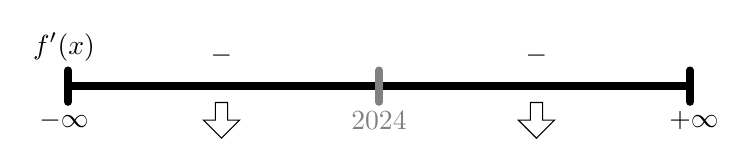
\begin{tikzpicture}[
                    every node/.style = {minimum size=1em,inner sep=2pt},
                         Arrow/.style = {single arrow, draw, minimum height=3ex, 
                                         single arrow head extend=1ex,
                                         shape border rotate=#1}
                                            ]
                    \draw[line width=1mm,{Bar[width=4mm,round]}-{Bar[width=4mm,round]}]
                        (0,0) node [above=2mm] {$f'(x)$} 
                              node [below=2mm] {$-\infty$}  -- ++ 
                        (8,0) node [above=2mm] {}
                              node [below=2mm] {$+\infty$} ;
                    \draw[line width=1mm,line cap=round,gray]
                        (4,-0.2) node[below] {$2024$} -- ++ (0,0.4);
                    % signs    
                    \node[above] at (2,0.2) {$-$};
                    \node[above] at (6,0.2) {$-$};
                    % arrows
                    \node[Arrow= 270, below] at (2,-0.2) {};
                    \node[Arrow= 270, below] at (6,-0.2) {};
                \end{tikzpicture}
            \end{center}
            $\therefore$ Fungsi $f(x)$ selalu turun pada selang $(-\infty, 2024)\cup(2024, +\infty)$.
            \item Karena $f'(x)$ tidak akan pernah nol, maka fungsi $f(x)$ tidak memiliki titik ekstrim.
            \item Tinjau turunan kedua dari $f(x)$
            \begin{align*}
                f''(x) &= \frac{d}{dx}\left(-\frac{2024}{(x-2024)^2}\right) = \frac{4048}{(x-2024)^3}
            \end{align*}
            Karena $f''(x) \neq 0$ untuk semua $x\in\R$, maka fungsi $f(x)$ tidak memiliki titik belok.\\
            Uji titik:
            \begin{itemize}
                \item $x = 0 \implies f''(0) = -\frac{2}{2024^2} < 0$.
                \item $x = 2025 \implies f''(2025) =  4048> 0$.
            \end{itemize}
            \begin{center}
                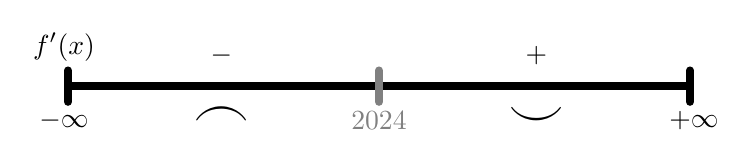
\begin{tikzpicture}[
                    every node/.style = {minimum size=1em,inner sep=2pt},
                         Arrow/.style = {single arrow, draw, minimum height=3ex, 
                                         single arrow head extend=1ex,
                                         shape border rotate=#1}
                                            ]
                    \draw[line width=1mm,{Bar[width=4mm,round]}-{Bar[width=4mm,round]}]
                        (0,0) node [above=2mm] {$f'(x)$} 
                              node [below=2mm] {$-\infty$}  -- ++ 
                        (8,0) node [above=2mm] {}
                              node [below=2mm] {$+\infty$} ;
                    \draw[line width=1mm,line cap=round,gray]
                        (4,-0.2) node[below] {$2024$} -- ++ (0,0.4);
                    % signs    
                    \node[above] at (2,0.2) {$-$};
                    \node[above] at (6,0.2) {$+$};
                    % arrows
                    \node[below] at (2,-0.2) {\huge$\frown$};
                    \node[below] at (6,-0.2) {\huge$\smile$};
                \end{tikzpicture}
            \end{center}
            $\therefore$ Fungsi $f(x)$ cekung ke bawah pada selang $(-\infty, 2024)$ dan cekung ke atas pada selang $(2024, +\infty)$.
            \item Dapat kita sketsa menggunakan informasi pergeseran grafik dari $f(x)=\dfrac{1}{x}$. (2024 satuan ke kanan dan 1 satuan ke atas)
            \begin{center}
                \begin{tikzpicture}[scale=0.8]
                    \draw [->] (-2,0) -- (7,0) node [right] {\footnotesize$x$};
                    \draw [->] (0,-2) -- (0,4) node [above] {\footnotesize$y$};
        
                    \draw [domain=4:7, samples=50, thick, blue] plot (\x, {\x/(\x-3)});
                    \draw [domain=-2:2, samples=50, thick, blue] plot (\x, {\x/(\x-3)});
                    \draw [domain=-2:4, samples=10, darkgray, dashed] plot (3, {\x});
                    \draw [domain=-2:7, samples=10, darkgray, dashed] plot ({\x}, 1);

                    \node [below right] at (3,0) {\footnotesize$2024$};
                    \node [below right] at (0,1) {\footnotesize$1$};
                \end{tikzpicture}
            \end{center}
        \end{enumerate}
        \item Untuk $F(-1)$, dapat dilihat karena nilai batas bawah dan batas atas sama, maka nilai integralnya adalah nol.
        \begin{flalign*}
            F(-1) &= \int_{-1}^{-1} \frac{1 + t^3}{1 + t^2} \, dt = 0&
        \end{flalign*}
        Selanjutnya untuk $F'(-1)$, dapat kita gunakan Teorema Fundamental Kalkulus II untuk mencari turunan dari $F(x)$.
        \begin{flalign*}
            F'(x) &= \frac{d}{dx}\left(\int_{-1}^x \frac{1 + t^3}{1 + t^2} \, dt\right) = \frac{1 + x^3}{1 + x^2}&\\
            F'(-1) &= \frac{1 + (-1)^3}{1 + (-1)^2} = 0&
        \end{flalign*}
        Terakhir untuk $F''(-1)$, kita turunkan $F'(x)$.
        \begin{flalign*}
            F''(x) &= \frac{d}{dx}\left(\frac{1 + x^3}{1 + x^2}\right) = \frac{3x^2(1 + x^2) - 2x(1 + x^3)}{(1 + x^2)^2}&\\
            F''(-1) &= \frac{3(-1)^2(1 + (-1)^2) - 2(-1)(1 + (-1)^3)}{(1 + (-1)^2)^2} = \frac{3(2)-0}{4}=\frac{3}{2}&
        \end{flalign*} 

        \item Agar lebih mudah dihitung, jadikan ketiga masing-masing bilangan kompleks diatas menjadi bentuk polar.
        \begin{itemize}
            \item Untuk $1+i$, didapatkan $a=1$ dan $b=1$ sehingga $r=\sqrt{1^2+1^2}=\sqrt{2}$ dan $\theta=\arctan\left(1\right)=\dfrac{\pi}{4}$ (Kuadran I).\footnote{Boleh dijadikan dalam bentuk derajat}
            \item Untuk $1+i\sqrt{3}$, didapatkan $a=1$ dan $b=\sqrt{3}$ sehingga $r=\sqrt{1^2+(\sqrt{3})^2}=2$ dan $\theta=\arctan\left(\sqrt{3}\right)=\dfrac{\pi}{3}$ (Kuadran I).
            \item Untuk $-1+i$, didapatkan $a=-1$ dan $b=1$ sehingga $r=\sqrt{(-1)^2+1^2}=\sqrt{2}$ dan $\theta=\arctan\left(-1\right)=\dfrac{3\pi}{4}$ (Kuadran II).
        \end{itemize}
        Jadi bentuk polar dari $z$ adalah
        \begin{align*}
            z&=\left(\frac{\left(1 + i\right)^{12}\left(1 + i\sqrt{3}\right)^{16}}{(-1 + i)^{32}}\right)=\frac{\left[\sqrt{2}\cis\left(\dfrac{\pi}{4}\right)\right]^{12}\left[2\cis\left(\dfrac{\pi}{3}\right)\right]^{16}}{\left[\sqrt{2}\cis\left(\dfrac{3\pi}{4}\right)\right]^{32}}=\frac{\left[2^{6}\cis\left(3\pi\right)\right]\left[\cancel{2^{16}}\cis\left(\dfrac{16\pi}{3}\right)\right]}{\cancel{2^{16}}\cis\left(24\pi\right)}\\
            &=\frac{\left[2^{6}\cis\left(\pi\right)\right]\left[\cis\left(\dfrac{4\pi}{3}\right)\right]}{\cis\left(0\right)}=2^{6}\cis\left(\pi+\dfrac{4\pi}{3}-0\right)=2^{6}\cis\left(\dfrac{7\pi}{3}\right)=2^{6}\cis\left(\dfrac{\pi}{3}\right)\\
            &=64\left(\cos\left(\dfrac{\pi}{3}\right)+i\sin\left(\dfrac{\pi}{3}\right)\right)=64\left(\dfrac{1}{2}+i\dfrac{\sqrt{3}}{2}\right)=\boxed{32+32\sqrt{3}i}
        \end{align*}
        \item Metode Cramer secara umum untuk mencari nilai $x_n$ dapat dirumuskan sebagai
        \[x_n=\frac{\det(A_n)}{\det(A)}\]
        dengan $A_n$ adalah matriks yang diperoleh dari matriks $A$ yang kolom ke-$n$-nya diganti dengan vektor kolom $b$. (Dalam hal ini $n=3$)

        SPL diatas dapat dituliskan dalam bentuk matriks sebagai berikut
        \[\underbrace{\begin{pmatrix}
            1 & 0 & 4 & 1\\
            2 & 0 & 3 & 2\\
            5 & 1 & 2 & 1\\
            4 & 0 & 6 & 1
        \end{pmatrix}}_{A}\underbrace{\begin{pmatrix}
            x_1\\x_2\\x_3\\x_4
        \end{pmatrix}}_{x}=\underbrace{\begin{pmatrix}
            11\\12\\20\\24
        \end{pmatrix}}_{b}\]
        Kemudian kita tulis matriks $A_3$ dengan mengganti kolom ke-3 dari matriks $A$ dengan vektor kolom $b$.
        \[A_3=\begin{pmatrix}
            1 & 0 & 11 & 1\\
            2 & 0 & 12 & 2\\
            5 & 1 & 20 & 1\\
            4 & 0 & 24 & 1
        \end{pmatrix}\]
        Selanjutnya kita hitung nilai determinan dari matriks $A$ dan $A_3$. Ada banyak metode untuk menghitung determinan, seperti OBE, ekspansi kofaktor, dsb. Disini saya akan menggunakan metode ekspansi kofaktor dan OBE.\footnote{OBE dan ekspansi kofaktor memang bisa di-\textit{combine} untuk mempercepat perhitungan}
        \begin{itemize}
            \item Untuk $\det(A)$, pertama akan kita ekspansi kofaktor sepanjang kolom kedua karena memiliki banyak nol.
            \begin{align*}
                \begin{vmatrix}
                    1 & 0 & 4 & 1\\
                    2 & 0 & 3 & 2\\
                    5 & 1 & 2 & 1\\
                    4 & 0 & 6 & 1
                \end{vmatrix}=-0...+0...-(1)\begin{vmatrix}
                    1 & 4 & 1\\
                    2 & 3 & 2\\
                    4 & 6 & 1
                \end{vmatrix}+0...=-\begin{vmatrix}
                    1 & 4 & 1\\
                    2 & 3 & 2\\
                    4 & 6 & 1
                \end{vmatrix}
            \end{align*}
            Untuk matrix $3\times 3$ kita bisa menggunakan aturan Sarrus, namun disini saya akan menggunakan OBE yaitu $B_2-2B_1$ dan $B_3-4B_1$.\footnote{OBE tipe ini tidak mengubah nilai determinan matriks awal}
            \begin{align*}
                -\begin{vmatrix}
                    1 & 4 & 1\\
                    2 & 3 & 2\\
                    4 & 6 & 1
                \end{vmatrix}&=-\begin{vmatrix}
                    1 & 4 & 1\\
                    0 & -5 & 0\\
                    0 & -10 & -3
                \end{vmatrix}=-\begin{vmatrix}
                    -5 & 0\\
                    -10 & -3
                \end{vmatrix}=-[(-5)(-3)-(-10)0]=-15
            \end{align*}
            \item Untuk $\det(A_3)$, dengan langkah yang sama kita ekspansi kofaktor sepanjang kolom kedua.
            \begin{align*}
                \begin{vmatrix}
                    1 & 0 & 11 & 1\\
                    2 & 0 & 12 & 2\\
                    5 & 1 & 20 & 1\\
                    4 & 0 & 24 & 1
                \end{vmatrix}=-0...+0...-(1)\begin{vmatrix}
                    1 & 11 & 1\\
                    2 & 12 & 2\\
                    4 & 24 & 1
                \end{vmatrix}+0...=-\begin{vmatrix}
                    1 & 11 & 1\\
                    2 & 12 & 2\\
                    4 & 24 & 1
                \end{vmatrix}
            \end{align*}
            Dan kita gunakan OBE yang sama yaitu $B_2-2B_1$ dan $B_3-4B_1$.
            \begin{align*}
                -\begin{vmatrix}
                    1 & 11 & 1\\
                    2 & 12 & 2\\
                    4 & 24 & 1
                \end{vmatrix}&=-\begin{vmatrix}
                    1 & 11 & 1\\
                    0 & -10 & 0\\
                    0 & -20 & -3
                \end{vmatrix}=-\begin{vmatrix}
                    -10 & 0\\
                    -20 & -3
                \end{vmatrix}=-[(-10)(-3)-(-20)0]=-30
            \end{align*}
        \end{itemize}
        Terakhir kita gunakan rumus Cramer untuk mencari nilai $x_3$.
        \[x_3=\frac{\det(A_3)}{\det(A)}=\frac{-30}{-15}=2\]
    \end{enumerate}
\end{document}